\chapter{Imaging methods}\label{ch4:Imaging-methods}
\begin{remark}{Outline}
\end{remark}

\section{Data management}\label{sec:image-data-management}
In 2013 monitoring image data were corrupted after hard-drive failures. Images were recovered using open source forensic tools, TestDisk\footnote{\emph{TestDisk} http://www.cgsecurity.org/wiki/TestDisk} and PhotoRec\footnote{\emph{TestDisk }http://www.cgsecurity.org/wiki/PhotoRec}. When the recovery process was finished the bash scripts shown in Listing \ref{cd:photorec} were run to restore images and a very basic folder structure. A complete folder structure was then created and used for monitoring image data. Folder templates were outlined and they remained consistent over all folders (Figure \ref{fig:folder}). To preserve original data, image operations were performed on duplicate folders (e.g. Folders 071\_~sort\_~collections and 018\_~sorted\_~collections). The workflow for each folder (any file or imaging procedures) was documented and saved in readme files. These were attached to base folders for reference. The folder names were chosen to be as short as possible, while remaining descriptive enough to follow. Batch processing techniques were applied to a \emph{copy} of a working folder before being used on final folders. The procedures used to restore the monitoring image database are summarised as follows:

\begin{enumerate}
\item Invoked TestDisk software to check if the partition table of the old drive could be restored; it was unrecoverable.
\item Invoked PhotoRec to restore raw data files from the failed drive to a new external hard-drive (2T byte). Copied the database onto a separate  back-up hard-drive (2T byte) using Grsync\footnote{\emph{Grsync} http://www.opbyte.it/grsync} file synchronization software tool. 
\item Restored the folder structure of the raw recovered data by using exiftool\footnote{\emph{exiftool} http://www.sno.phy.queensu.ca/~ phil/exiftool} \cite{Exiftool2013} and the bash scripting shown in Listing \ref{cd:photorec} below.
\item Created the final folder structure for monitoring data, shown in Figure \ref{fig:folder} below.

\begin{lstlisting}[float, language=bash, caption={[Bash script.]Bash script to sort Photorec recovered images by extension; and into date-time based folders.}, label=cd:photorec]
#Copy images of a certain type/size into a new folder
#!/bin/bash
recup_dir="${1%/}" [ -d "$recup_dir" ] || 
{echo "Usage: $0 recup_dir"; echo "Mirror files from recup_dir into recup_dir.by_ext, organized by extension"; exit 1};
find "$recup_dir" -type f | while read k; do
ext="${k##*.}"; ext_dir="$recup_dir.by_ext/$ext";
[ -d "$ext_dir" ] || mkdir -p "$ext_dir";
echo "${k%/*}" ln "$k" "$ext_dir"; done

#Sort images into newly created date-time based folders.
$w_dir = '/home/nh/ext_dir';
$r_dir = '/home/nh/photos/'
$jhead_bin = '/usr/bin/jhead';
@rec_dirs = `ls ${w_dir} | grep recup_dir`;
foreach $recup_dir (@rec_dirs) {print "Scanning ${recup_dir}...";
chomp $recup_dir;
@photos_in_recup = `find ${w_dir}${recup_dir}/*jpg -type f -size +800k`;
foreach $photo_file (@photos_in_recup) 
{chomp $photo_file; print "IMG $photo_file in $recup_dir\n";
@exif = `$jhead_bin -v $photo_file`;
print "$jhead_bin -v $photo_file\n";
foreach $line (@exif) {if ($line =~ /Time\s*:\s*([0-9]{4}):([0-9]{2}):([0-9]{2})\s[0-9:]{8}$/) {print "IMG $photo_file $1-$2-$3\n"; 
system("mkdir ${r_dir}$1-$2-$3"); 
system("mv $photo_file $r_dir/$1-$2-$3/");last; }}}}
\end{lstlisting}
\end{enumerate}

\begin{figure}[!htbp]\myfloatalign
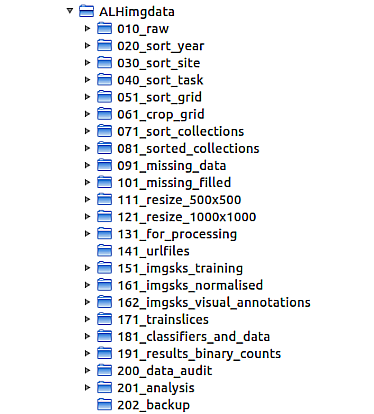
\includegraphics[width=.6\linewidth]{gfx5/prep/folder}\\
\caption[Folder structure for image database.]{Folder structure created for the monitoring image database.}\label{fig:folder}
\end{figure}

\section{Computing environment}
A Linux operating system was used. It was configured for the specific image monitoring tasks and to mitigate memory leaks during classifications. Ubuntu (14.04) swap memory was turned off during image processing tasks to prevent processes from swapping out of physical memory. Virtual memory\footnote{refer to: http://docs.oracle.com/cd/E13222\_01/wls/docs81/perform/JVMTuning.html} options were also passed to JavaVM from \acs{Fiji}'s main configuration file to increase the memory heap size. These settings are shown in Listing \ref{cd:java} below. Image data were processed on standard computer. There system specifications are listed in Table \ref{tab:pcspecs} below.

\begin{table}[!htbp] \myfloatalign \caption[Computer specifications.]{Computer hardware and operating system specifications.}\label{tab:pcspecs} 
\begin{tabular}{p{2.1in}p{2.3in}} \\ \toprule
Operating system & Ubuntu 14.04\\
Linux kernel & 3.13.0-48-generic\\
PC & CQ1-1240IN Desktop PC \\
Monitor & 46.99cm LCD\\
Ram & 7.4 GiB\\
Processor&  2 x AMD E-350\\
Graphics card &  Gallium 0.4 on AMD PALM\\
Java(TM) & java.runtime.version 1.6.0\_24-b07\\
\acs{Weka} & version	3.7.11\\
Fiji/ImageJ & 1.49u \\ \bottomrule
\end{tabular}
\end{table}

\begin{lstlisting}[language=bash, caption={[Operating system configuration.]JavaVM memory options passed from Fiji's configuration files; and Ubuntu swap memory and cache adjustments. These were made to improve the stability of the operating system for image processing tasks.}, label=cd:java]
#JavaVM options passed from Fiji configuration file.
------------------------------------------
jre/bin/java -Xms3000m -Xmx4000m -Xincgc -cp -XX:MaxPermSize=256m -XX:PermSize=256m -XX:NewRatio=5 -XX:CMSTriggerRatio=20 -XX:+UseCompressedOops -XX:+UseParNewGC -XX:MinHeapFreeRatio=5 -XX:MaxHeapFreeRatio=10 -- ij.jar ij.ImageJ
------------------------------------------
#Bash script to turn off linux memory swap
------------------------------------------
cat /proc/sys/vm/swappiness
gksudo leafpad /etc/sysctl.conf
# Decrease swap usage to a more reasonable level--or turn off
vm.swappiness=10
# Improve cache management
vm.vfs_cache_pressure=50
------------------------------------------
\end{lstlisting}

\section{Image preparation}\label{sec:image-preparation}

More than one category of images were collected during monitoring. These included photographs of a) bees in flight or foraging, b) active nests with and without a standard grid measure, c) active nests acquired with a Smart Phone, d) a range of monitoring videos. Raw data were therefore sorted by year, site and image monitoring-\emph{task}. Images of active nests using a grid standard of measure are used in this analysis. These images were sorted by year, site, and grid number (1--4). The preparation of image data for active nests are listed as follows:

\begin{itemize}
\item Active nest images were sorted to year, site, grid-folders (Figure \ref{fig:preparation} (a)). 
\item Images were renamed using Xnview (Figure \ref{fig:preparation} (b)).
\item Image exif metadata was combined with the sub-folder grid identifier to create unique file name identifiers.
\item Nest images were cropped to a square grid using Xnview (Figure \ref{fig:preparation} (c)).
\end{itemize}

\begin{figure}[!htbp]\myfloatalign
\subfloat[Raw images sorted.]{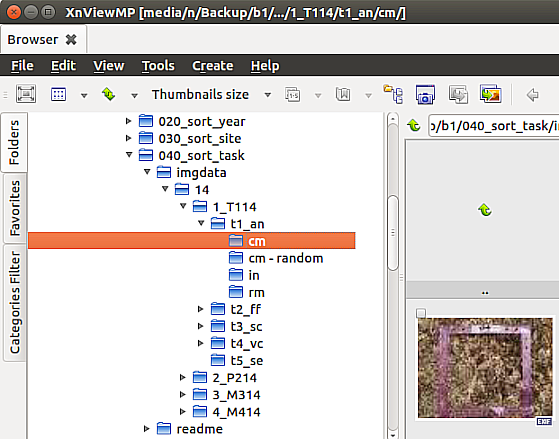
\includegraphics[width=0.35\linewidth]{gfx5/prep/sorttype}}\
\subfloat[Renamed with Xnview.]{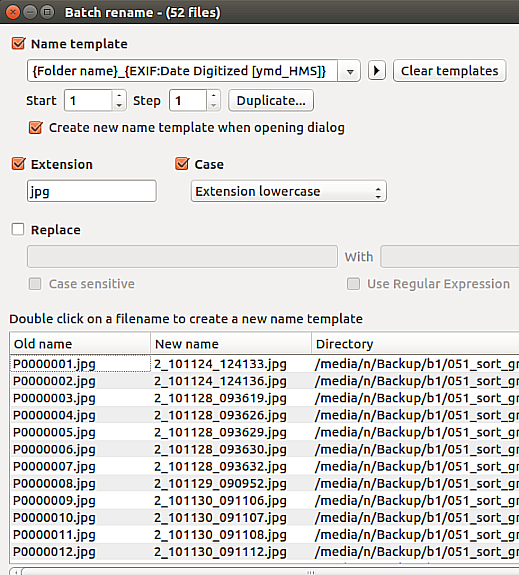
\includegraphics[width=0.3\linewidth]{gfx5/prep/rename}}\\
\subfloat[Nest images cropped.]{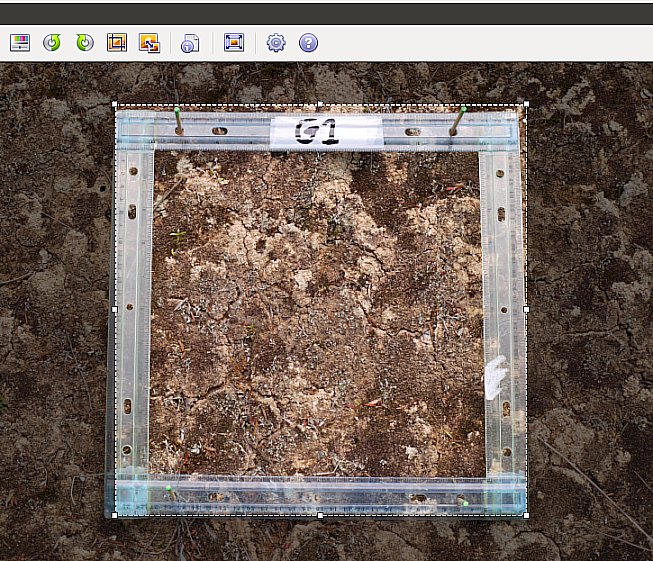
\includegraphics[width=0.35\linewidth]{gfx5/prep/crop}}\\
\caption[Image preparation.]{Preparation of monitoring data. Nest images (a) acquired using a constructed standard of measure (cm) are used in this analysis. Active nest images were (b) sorted to grids and renamed and (c) cropped to the outside grid using XnView software.}\label{fig:preparation}
\end{figure}

\clearpage

\subsection{Sorting image collections}\label{sec:sorting-image-collections}
The images of active nests were manually cropped to the outside grid edge using XnView as shown in Figure \ref{fig:preparation} (c). Once cropped, images were sorted into separate \emph{collections}. Collections were image sequences of the same nest, separated by minutes-seconds. Collections were sorted into four folders; C1--C3 were used in analysis and C4 contained all/or any other extra images. The following procedure was used to automatically sort images into collections:

\begin{enumerate}
\item Images were cropped (Figure \ref{fig:preparation} (c)) and saved to Folder \\
/061\_~crop\_~grid before sorting.
\item XnView catalogue feature \emph{Create > File listing} was used to create a list.csv file (Figure \ref{fig:sort} (a)).
\begin{enumerate}
	\item The list.csv file was used to organise yearly data.
	\item Exif metadata data-time information were displayed for each image.
		\begin{figure}[!htbp]\myfloatalign
		\subfloat[XnView file list.]{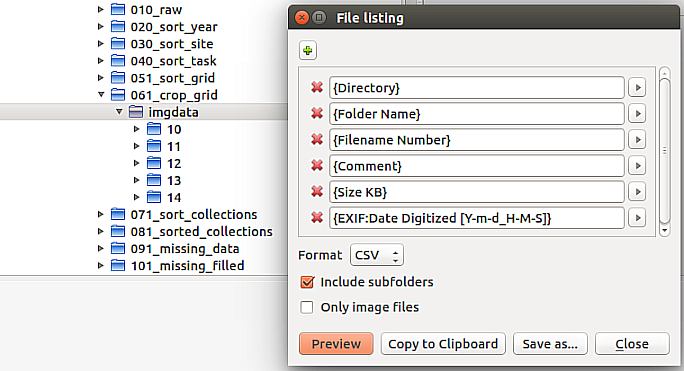
\includegraphics[width=.7\linewidth]{gfx5/prep/xnview-filelist}}\\
		\subfloat[CSV file listings.]{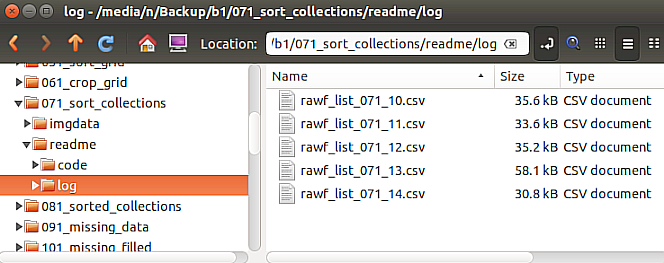
\includegraphics[width=.7\linewidth]{gfx5/prep/csv-filelist}}\\
		\subfloat[Sorting image collections.]{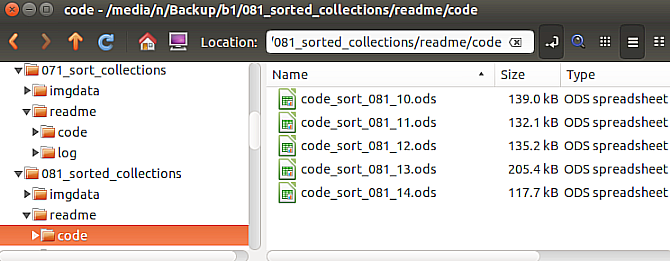
\includegraphics[width=.7\linewidth]{gfx5/prep/ods-sort}}\\
		\caption[File organising and procedures.]{Organising data by (a) XnView file listings, (b) CSV file lists  and (c) Open Office Cal spreadsheets used to sort image collections. }\label{fig:sort}
		\end{figure}
\end{enumerate}
\item The list.csv file was imported into Apache OpenOffice Calc\footnote{https://www.openoffice.org/} (Figure \ref{fig:sort} (b)).
	\begin{enumerate}
	\item Date-time attributes of each image were used to sort data into four separate collections.
	\item The Calc spreadsheet (Figure \ref{fig:sort} (c) above) was used to write a bash script to:
	\begin{enumerate}
	\item Copy images from the source directory.
	\item Save images to the predefined destination directory with subfolders: C1, C2, C3 and C4.
	\end{enumerate}
	\end{enumerate}
\begin{enumerate}
\item The exif information for each images was retained during the copying process with exiftool, as shown in Listing snippet \ref{cd:sort} below.

\begin{lstlisting}[language=bash, caption=Bash snippet to sort collections., label=cd:sort]
#Use exiftool -tagsFromFile to get tages from files...cp copy from DIR - to DIR#
ref_id	//copy exif tags//copy_from Dir //save_to Dir
exiftool -tagsFromFile cp /ALHimgdata/071_sort_collections/imgdata/10/1_T110ANCM/C1/1/1_101124_124112.jpg
/ALHimgdata/081_sorted_collections/imgdata/10/1_T110ANCM/C1/1C1/1C1_101124_124112_1.jpg
exiftool -tagsFromFile cp /ALHimgdata/071_sort_collections/imgdata/10/1_T110ANCM/C1/1/1_101124_124113.jpg /ALHimgdata/081_sorted_collections/imgdata/10/1_T110ANCM/C2/1C2/1C2_101124_124113_2.jpg
\end{lstlisting}
\end{enumerate}
\item Once the process was completed the file numbers were reviewed via XnView file listings to ensure the correct number of files had been copied.
\item Note: This sorting process was repeated to select training images for training stacks (Figure \ref{fig:sortselecttrain} (a)). 
	\begin{enumerate}
	\item The list.csv was imported into Apache OpenOffice Cal and used to select the third or fourth monitoring day for each year, site and grid.
	\item The final list was written into a bash script.
	\item The script automatically copied images from the processing folder (131\_for\_ processing) to the training stacks folder  (151\_imgsks\_ training) as shown in Figure \ref{fig:sortselecttrain} (b).
\end{enumerate}
\item Filler data (ND) were created monitoring images as shown in Figure \ref{fig:sortselecttrain} (c).
	\begin{enumerate}
	\item A white image was labelled with ND and copied.
	\item The exif date-time, and name of each filler image was changed to match the monitoring collections.
	\item Filler images were selected, copied and pasted into folder (101\_missing\_ filled) using Ubuntu merge.
	\item  Existing images were not overwritten and only images representing \emph{missing} files were copied.
	\end{enumerate}
\end{enumerate}

\begin{figure}[!htbp]\myfloatalign
\subfloat[Sorting image collections (C1--C3).]{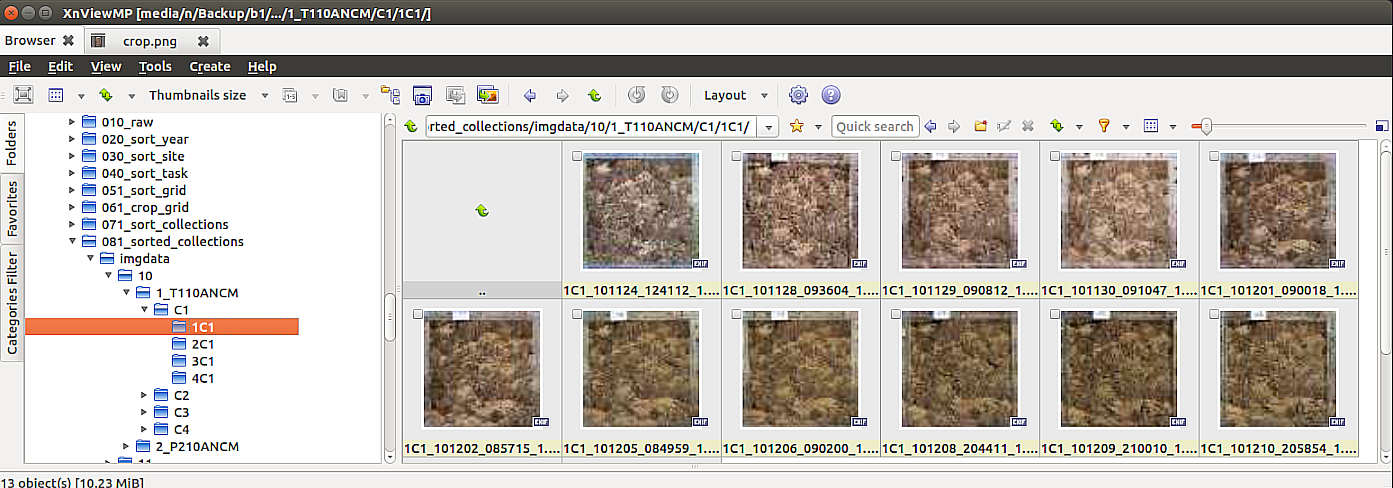
\includegraphics[width=.9\linewidth]{gfx5/prep/sortcollections}} \\
\subfloat[Selecting training slices for training stacks.]{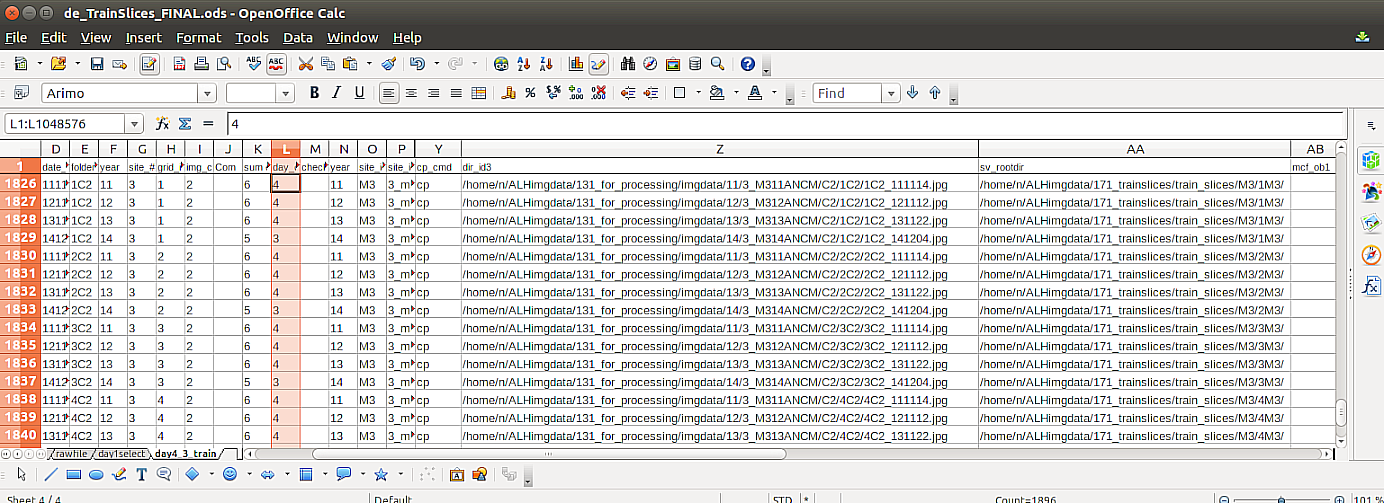
\includegraphics[width=.9\linewidth]{gfx5/prep/selecttrain}} \\
\subfloat[Filler image files added to monitoring data.]{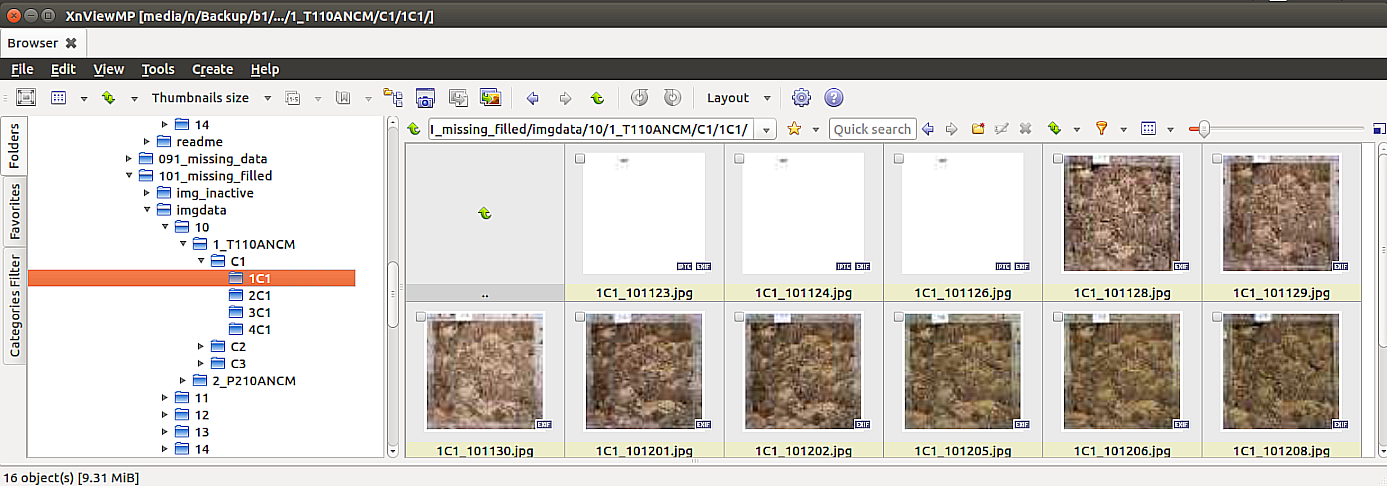
\includegraphics[width=.9\linewidth]{gfx5/prep/filler}} \\
\caption[Sorting image collections.]{File methods for (a) sorting image collections and (b) selecting training slices (c) filling missing image fills with ND data.}\label{fig:sortselecttrain}
\end{figure}

\subsection{Pre-processing procedures}\label{sec:pre-processing-procedures}
Pre-processing procedures are summarised briefly below. Classification methods are outlined generally but techniques are examined in more detail in the proceeding Sections.

\begin{enumerate}
\item Images were cropped to the outside grid.
\item They were resized to 500 x 500 pixels.
\begin{enumerate}
\item Bicubic interpolation was selected for resizing.
\item It produces smoother images with fewer interpolation artefacts.
\item Chosen over other methods since speed was not an issue. 
\end{enumerate}
using bicubic interpolation\footnote{Bicubic interpolation was chosen over other methods since speed was not an issue. Bicubic interpolation produces smoother images with fewer interpolation artefacts}.
\item Monitoring images were collated into time based stacks.
	\begin{enumerate}
	\item Stacks were saved in .tiff format.
	\item Example script snippet in Listing \ref{cd:collate-images-into-stacks} below:
\begin{lstlisting}[language=bash, caption=Collate images into stacks, label=cd:collate-images-into-stacks]
run("Image Sequence..."," open=[t110_1c1] convert_to_rgb sort");
saveAs("TIFF",st110_1c1+"st110_1c1");
\end{lstlisting}
	\end{enumerate}
\item Images were enhanced using \emph{contrast enhancement} to improve visual appearance.
	\begin{enumerate}
	\item Saturated pixels were set to 0.4\%.
	\item Each slice was enhanced.
	\item Example script snippet in Listing \ref{cd:enhance-image-contrast} below:
\begin{lstlisting}[language=bash, caption=Enhance image contrast, label=cd:enhance-image-contrast]
run("Enhance Contrast...", "saturated=0.4 process_all");
saveAs("Tiff", "/161\_imgsks\_normalised/imgsks/s10/1\_t1/st110\_1c1.tif");
\end{lstlisting}
	\end{enumerate}
\end{enumerate}


\subsection{Overview of file and folder procedures }\label{sec:overview-of-procedures-by-folder}
The following paragraphs provide a general overview of practical procedures used throughout the imaging pipeline. Each important processing *task will be discussed in greater detail in Sections \ref{sec:classifier-training} and \ref{sec:post-processing}. Several common files types are discussed in this Chapter so are briefly listed first for clarity:

\begin{itemize}
\item IJM: ImageJ Macro--a scripting language to automate processing.
\item ARFF: Attribute-Relation File Format--an ASCII text file that describes a list of instances sharing a set of attributes; used in \ac{TWS} and \ac{Weka}.
\item MODEL: Model--\ac{Weka} classifier model file; once trained and constructed the model can be saved and reloaded for application; used in \ac{TWS} and \ac{Weka}.
\item R: R file--script written in R for statistical analysis.
\item CSV: Comma Separated Value--for statistical analysis in R-studio.
\item ODS: Open Document Spreadsheet--for raw data entry in Apache Open Office.
\item TXT: Text--plain text output log from \ac{TWS} and \ac{Weka}.
\end{itemize}

\paragraph{Folder 061\_crop\_grid:} Image data were manually cropped to grids using XnView.

\paragraph{Folders 071\_sort\_collections} and Folder 081\_sorted\_collections: Image data were sorted into separated image collections. These processes are explained further in Section \ref{sec:sorting-image-collections} 

\paragraph{Folder 101\_missing\_filled:} Filler image data were added to folders to retain the sequential order of image collection monitoring days. This was necessary since some image data were not recovered from the hard-drive failure.

\paragraph{Folder 111\_resize\_500x500:} Images were resized to upload to the GitHub database.

\paragraph{Folder 121\_resize\_1000x1000:} Images were resized for visual annotation and checking.

\paragraph{*Folder131\_for\_processing:} Image data for pre-processing were stored in this folder.

\paragraph{Folder141\_urlfiles:} Image data were renamed for uploading to online databases. 

\paragraph{*Folder 151\_imgsks\_training:} Images were collated by \ac{Fiji} macro into image stacks for processing and saved as .tiff files. All macro (.ijm) and images stacks (.tiff) were stored in this folder.

\paragraph{*Folder 161\_imgsks\_normalised} Stacks were enhanced with $0.4\%$ saturated pixels.

\paragraph{Folder 162\_imgsks\_visual\_annotations} Image data used for visual annotations were saved to this folder including any image overlays.

\paragraph{*Folder 171\_trainslices} All training stacks were stored in this folder, including the \emph{control image} and the \emph{inactive nest} images for respective grids. These processes are explained further in Section \ref{sec:training-stacks}.

\paragraph{*Folder 181\_classifiers\_data} All training stacks and output files were stored in this folder. This included final annotation data (.arff), classifier models (.model), training log files (.csv and .txt) and final classified images (.tiff). The folder was structured per site and grid. With subfolders for each grid (1,2,3 and 4) within each of the site folders M3, P2 and T1 as shown below. These processes are explained further in Section \ref{sec:classifier-training}.

\begin{enumerate}
\item log\_final: When respective segmentations were satisfactory then final classifiers were applied to all image stacks and a log file (.txt) of final classifications is saved for records.
\item results: Binary image results were stored in this folder.
\item stacks: Image stacks for processing were stored in this folder.
\item data: Classifiers (.model), data files (.arff), training logs (.txt) and training binary image results (.tiff) were stored in this folder. The final training macro file for each grid was also stored in this folder. The macros used in the first training runs were stored in separate respective subfolders for reference.
\end{enumerate}

\paragraph{*Folder 191\_results\_binary\_counts} Post-processing image data (.tif), macro files (.ijm) and results (.txt and .csv) were stored in this folder. Post processing operations included cropping images, applying morphological operators and counting binary image objects based on their size and shape.

\section{Trainable segmentation interface}\label{sec:segmentation-interface}
Trainable Weka Segmentation user interface and options are shown in the Figures \ref{fig:twsgui}, \ref{fig:guifeatures} and \ref{fig:guioptions} below. They are intemperately referred to in later sections regarding  classifier testing and training methods, and the models created for nest images. The main user interface and script editor are shown in Figures \ref{fig:twsgui} (a)--(b). Feature settings and options for classifiers are shown in Figure \ref{fig:guifeatures}. Finally \ac{Weka} model options and model information interfaces are shown in Figures \ref{fig:guioptions}

\begin{figure}[!htbp]\myfloatalign
\subfloat[Test stack of images showing training for slice 1 of 6. Two traces are selected to represent class 1 and 2.]{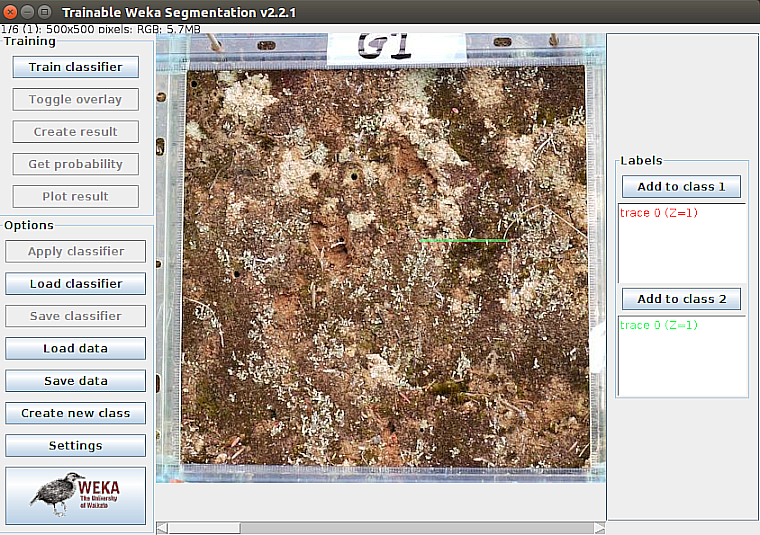
\includegraphics[width=0.9\linewidth]{gfx5/ctest/twsmain}}\\
\subfloat[\ac{Fiji} script editor: with the classifier test macro (ijm) loaded.]{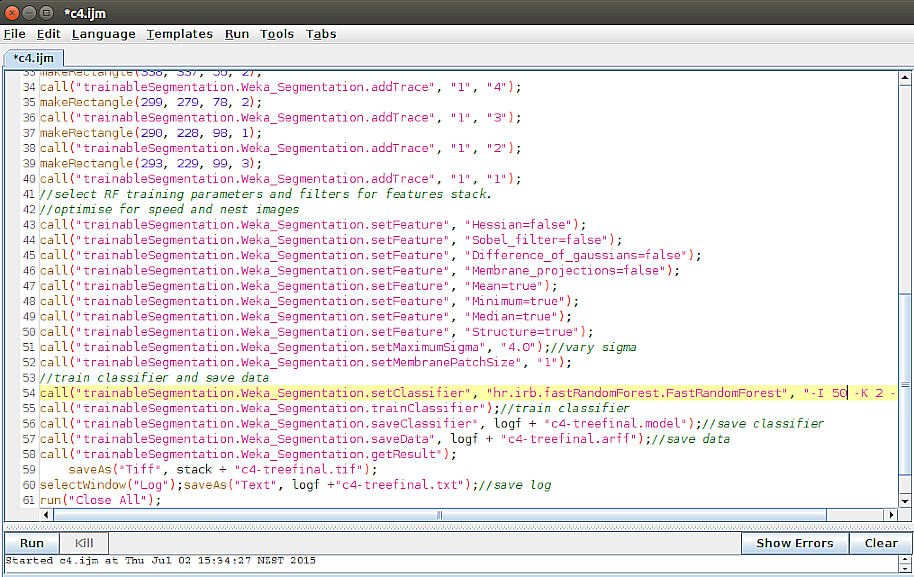
\includegraphics[width=0.9\linewidth]{gfx5/ctest/macro}}\\
\caption[\ac{TWS} main training interface.]{\ac{TWS} (a) graphical user interface (b) the script editor.}\label{fig:twsgui}
\end{figure}
\begin{figure}[!htbp]\myfloatalign
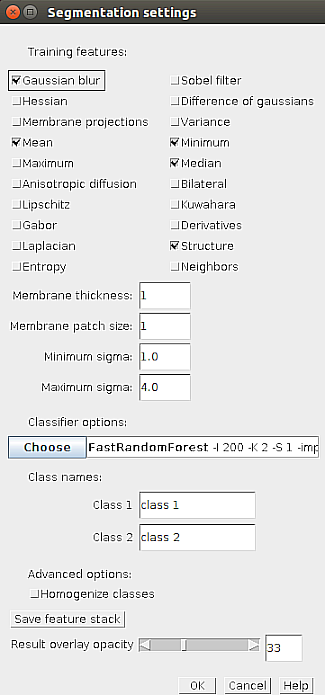
\includegraphics[width=0.36\linewidth]{gfx5/ctest/twss} \\
\caption[\ac{TWS} features settings interface.]{\ac{TWS} features settings interface.}\label{fig:guifeatures}
\end{figure}
\begin{figure}[!htbp]\myfloatalign
\subfloat[Model options.]{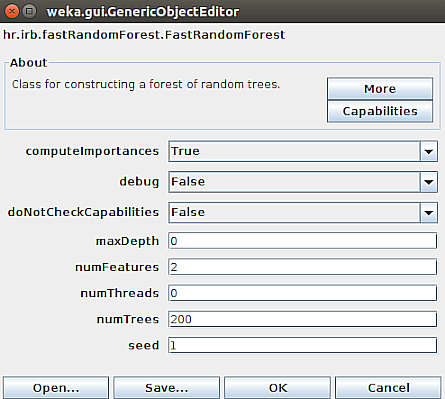
\includegraphics[width=0.45\linewidth]{gfx5/ctest/options}} \ \subfloat[Model information]{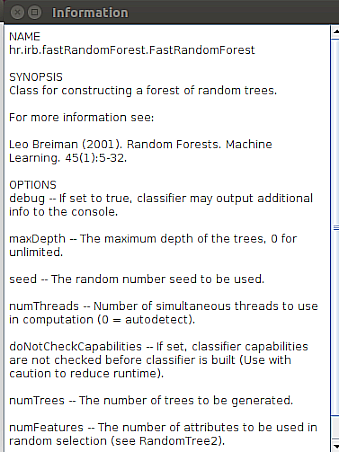
\includegraphics[width=0.31\linewidth]{gfx5/ctest/optionsinfo}} \
\caption[\ac{TWS} model options interface.]{\ac{TWS}, (a) the model option settings and (b) information about the Weka model}\label{fig:guioptions}
\end{figure}

\subsection{Filter descriptions and setting options}\label{sec:filter-descriptions}
The filter listed below are used in classifier tuning tests. They were selected from a possible twenty, to highlight the textural information in images of active nests. A brief description of each is included here for reference.

\begin{enumerate}
\item \emph{Mean, Variance, Median, Minimum, Maximum}. The pixels within a radius of $ 1, 2, 4 ... 2n $ pixels from the target pixel are subjected to the mean, variance, median, minimum and maximum operation; the target pixel is then set to that value. 
\item \emph{Structure filter}. For all elements in the input image this filter calculates the eigenvalues (smallest and largest) of the structure tensor also referred to as the second-moment matrix. The matrix is derived from the gradient of a function. It summarizes the predominant directions of the gradient in a specified neighbourhood of a point, and the degree to which those directions are coherent \cite{Meijering2007}. It uses a smoothing scale with $\sigma = 1, 2, 4...2n$ and integration scales $1$ and $3$.
\item \emph{Difference of gaussians}. Operator performs $ n $ individual convolutions with Gaussian kernels with $\sigma = 1, 2, 4... 2n$. The larger the radius the more blurred the image becomes until the pixels are homogeneous. By default $ n = 4 $, therefore $ = 1, 2, 4, 8$ and $16$. 
\item {Membrane projections}. Sobel filter calculates the intensity values in a 3 x 3 region around each image point to approximate the corresponding image gradient. In \ac{TWS} a Gaussian blur operator with $\sigma = 1, 2, 4... 2n $ is performed prior to the Sobel operator.
\item \emph{{Anisotropic diffusion}}. Filtering with 20 iterations $1, 2, 4, ... 2n$ smoothing per iterations and an edge threshold set to the membrane size \cite{Tschumperle2005}.
\item \emph{Bilateral filter}. Preserves edges while averaging other parts of the image and is similar to the Mean filter \cite{Chaudhury2011}. It accomplishes
blurring by only averaging the values around the current pixel that are close
in colour value to the current pixel. The closeness of other neighbourhood
pixels to the current pixels is determined by the specified threshold. For example with a value set to 10 each pixel that contributes to the current
mean has to be within 10 values of the current pixel. In \ac{TWS} this is a
combination of spatial radii of 5, 10 and 20, with a range radius of 50 and
100.
\item \emph{Lipschitz filter}. A Lipschitz cover of an image is equivalent to a
greyscale opening by a cone. The cover can be applied for the elimination of a slowly varying image background by subtraction of the lower Lipschitz cover (a top-hat procedure) \cite{Vstencel2006}. 
\item \emph{Kuwahara filter}. A noise-reduction filter that preserves edges. In \ac{Fiji}, the version of Kuwahara filter uses linear kernels rather than square. With a membrane patch size, as the kernel size and 30 angles and 0, 1 and 2.
\item There are four filter options used in the trainable segmentation set-up and tests. These are briefly described. Only the values of sigma were adjusted for nest segmentations and classifier testing. The other settings mentioned relate to biological image analysis and were not used for nest image processing.
\begin{itemize}
\item {Membrane thickness} is the expected value of the membrane thickness 1 pixel by default. This setting was not used for nest analysis and pertains to the membrane thickness of biological cells (e.g. brain image scans).
\item {Membrane patch size} represents the size $ NxN $ of the field of view for the membrane projection filters. This setting was not used for nest analysis and pertains to the membrane thickness of biological cells (e.g. brain image scans).
\item {Minimum sigma} the minimum radius of the filters used to create the features. By default is 1 pixel. For classifier optimisation testing and nest image analysis $\sigma_{min} = 1$
\item {Maximum sigma} the maximum radius of the filters used to create the features. By default is 16 pixels. For classifier optimisation testing and nest image analysis $\sigma_{max} = 2-16$.
\end{itemize}
\end{enumerate}

\section{Classifier tuning}\label{sec:classifier-tuning}
Six images of active nests were selected for classifier optimisation tests. Nest images (Figure \ref{fig:repstack}) were chosen to represent the full variation of monitoring data. A macro script was written to automate the testing; this is shown in Figure \ref{fig:twsgui} (b). User-traces were saved as rep\_nest.arff, so the same feature vectors could be applied to all classifier models during evaluations (see Figure \ref{fig:twsgui} (a)). Small repetitive tests were applied to a stack of representative nest images. This was to examine the affects of filters on classifications and image segmentations. Tests were also designed to investigate classifier performance and the affects on segmentations when model parameters were adjusted. Tests are outlined in Table \ref{tab:test-classifier-models} below and are detailed in the proceeding Sections.

\begin{figure}[!htbp]\myfloatalign
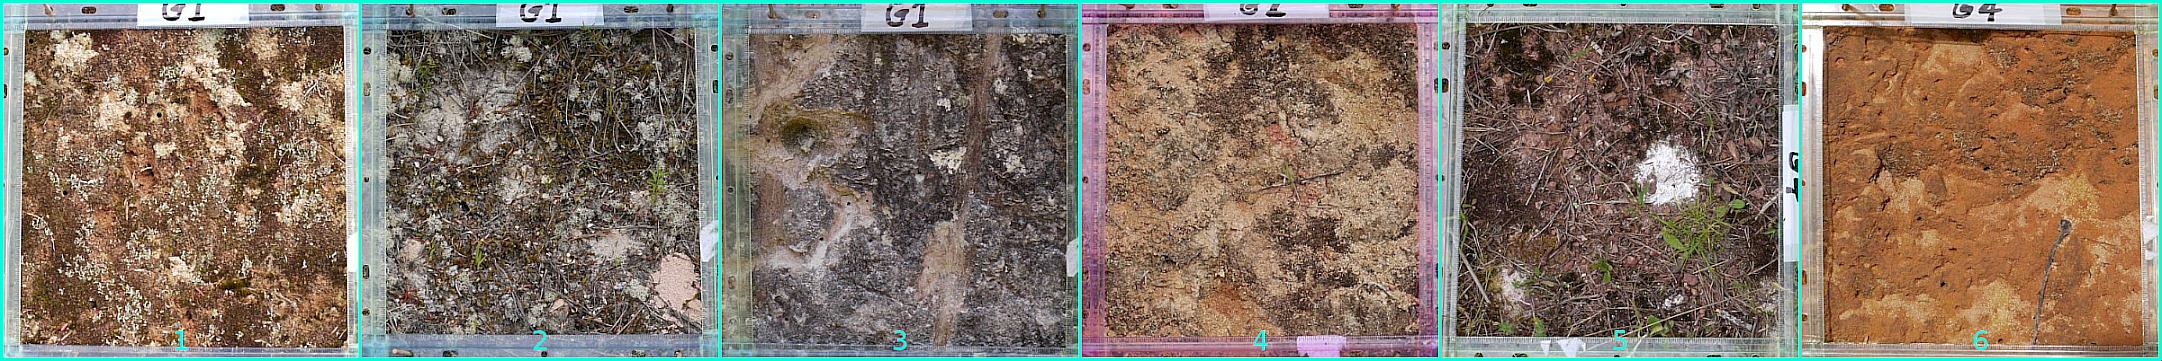
\includegraphics[width=1\linewidth]{gfx5/train/1rf} \\
\caption[Stack of representative images.]{Stack of representative images (slices 1--6) used to tune classifiers.}\label{fig:repstack}
\end{figure}


\begin{table}[!htbp] \myfloatalign \caption[Test classifier models.]{Test classifier models (T1--T5). The classifier model identifier (C1--C5) and the number of features in the stack created from the selected filters ($F_{n}$). The number of trees ($N$) used in tests and the number of random features used ($M$). The maximum value of sigma ($\sigma_{max}$) selected for tests. }\label{tab:test-classifier-models} 
\begin{tabular}{llllllp{2in}} \\ \toprule
Test & ID & $ F_{n} $ & $ N $ & $ M $ & $\sigma_{max}$ & Comment \\ \midrule
T1& C1 & 79 & 200 & 2 & $ 16 $ & Results from \ac{TWS} tests when default \ac{RF} settings are used. \\
T2& C2 & 46 & 200 & 2 & $ 4 $ & Results from \ac{TWS} tests when filters are optimised for best segmentation of nest images\\
T3& C3 & 20 & 200 & 2 & $ 2 $ & Results from \ac{TWS} tests when filters removed to reduce processing time.\\
T4& C4 & 20 & 10-1000 & 2 & $ 2 $ & Results from \ac{Weka} tests used to optimise number of trees.\\
T5& C5 & 20 & 50 & 0-20 & $ 2 $ & Results from \ac{Weka} tests used to optimise number of random features.\\
\bottomrule
\end{tabular}
\end{table}

\subsection{Testing feature importances}\label{sec:testing-feature-importances}

To evaluate the contribution of each filter $computeimportances$ was selected in the \ac{TWS} segmentation settings dialogue as shown in Figure \ref{fig:guioptions} (a).
The depth of tree growth $maxdepth$ was not checked and the model was permitted to grown to the maximum depth required during training. For each test the \ac{TWS} model output performance parameters including the: 1) feature importances, 2) time to create features stack and 3) the out of bag errors were saved as T$_{n}$.csv. Results were imported into an Apache Open Office spreadsheet for analysis.

During testing the filters that did not obviously contribute to the accuracy of final classifiers were removed; the training was re-run. The segmentation results were checked by comparing post-processed binary nest counts against raw \ac{RGB} images and manual nest counts taken in the field. This process was repeated until images from each representative slice were sufficiently segmented using the \emph{very minimum} number of features possible. The following tests were performed: 

\begin{enumerate}
\item Default features: Test 1
	\begin{itemize}
	\item Classifier C1 was not tuned, the default parameters were used.
	\item The filters selected were: Guassian blur, Sobel filter, Hessian, Difference of gaussians, and Membrane projections. 
	\item $F_n = 79$,  $N = 200$, $M = 2$ and $\sigma_{max} = 16$.
	\end{itemize}
\item Optimised features: Test 2
	\begin{itemize}
	\item Classifier C2 was tuned for features to enhance textural information. 
	\item The filters selected were: Guassian blur, Mean, Minimum, Median, Anisotropic diffusion, Bilateral, Lipschitz, Kuwahara and Structures. 
	\item $F_n = 46$, $N = 200$, $M = 2$ and $\sigma_{max} = 4$. 
	\end{itemize}
\item Optimised features: Test 3
	\begin{itemize}
	\item Classifier C3 was tuned to optimise the speed of feature stack creation, classifier training, construction and application. 
	\item The filters selected were: Gaussian blur, Mean, Minimum, Median and Structures. 
	\item $F_n = 20$, $N = 200$, $M = 2$ and $\sigma_{max} = 2$. 
	\end{itemize}
\end{enumerate}

\subsection{Testing random forest parameters}\label{sec:random-forest-parameters}

The number of trees in a forest should be initially set to 200; the initial number of random features is the square root of the maximum number of features. In the feature optimised test (C3) there were 20 features that were all important and contributed towards final classifications. Based on these tests the ideal number of random features was 5. \ac{RF} model parameters were adjusted to incorporate these ranges. The rep\_nest.arff dataset was used to evaluate the performances of models in \ac{Weka} Experimenter.

In test 4, twenty two \ac{RF} models were loaded into Algorithms for testing and the experiment was saved for repeat investigations as trees.exp. A 10 fold cross validation with a maximum of 10 iterations were selected for tests and used in the analysis. The number of trees were adjusted $N = 10-1000$ in each of the \ac{RF} models (with $F_n = 20$, $M = 2$ and $\sigma_{max} = 2$) and the analysis was run. The results from the experiment were saved in trees.arff and analysed in Weka. The out of bag error and overall time to complete processing was evaluated in \ac{TWS}. The output performance results were saved as tws\_trees.csv for analysis.

In test 5, twenty \ac{RF} models were added to Algorithms for testing and the experiment was saved for repeat investigations as random\_features.exp. A 10 fold cross validation with a maximum of 10 iterations were selected for tests and used in the analysis. The number of random features were adjusted between $ M = 0-20$ in each of the \ac{RF} models with $F_n = 20$, $N = 50$ and $\sigma_{max} = 2$. The analysis was run. The results from the experiment were saved as random-feature.arff and analysed in Weka. The out of bag error and overall time to complete processing was evaluated via \ac{TWS} and the output performance results were saved as tws\_random\_feature.csv for analysis. The procedures used in random forest parameter optimisation experiments are summarised as follows:

\begin{enumerate}
\item Optimal number of trees: Test $4_{N}$
	\begin{itemize}
	\item Classifier C4, twenty two \ac{RF} models were loaded into \ac{Weka} experimenter algorithms.
	\item The number of trees for each model was varied between $N = 10-1000$.
	\item With the other \ac{RF} parameters set at $F_n = 20$, $M = 2$ and $\sigma_{max} = 2$. 
	\end{itemize}
\item Optimal number of random features: Test $5_{M}$
	\begin{itemize}
	\item Classifier C5, twenty \ac{RF} models were loaded into \ac{Weka} experimenter algorithms.
	\item The number of random features for each model was varied between $M = 0-20$.
	\item With the other \ac{RF} parameters set at $F_n = 20$ $N = 50$ and $\sigma_{max} = 2$. 
	\end{itemize}
\end{enumerate}

\subsection{Classifier benchmarks}\label{sec:classifier-benchmarks}

The test classifier CF was compared against other well known machine learners in a final analysis. Several \ac{RF} classifiers were tested including the \ac{Weka} default model (M5), the \ac{Fiji} default model (M7),  a random feature optimised model (M6) and the final classifier CF model (M1). Six other common machine learners were tested including the zero rules model (M2), the J48 decision tree (M3), a random tree (M4), a Naive Bayes model (M8), a Voted Perception neural network (M9), and the SMO support vector model (M10).

A 10 fold cross validation with a maximum of 10 iterations were selected for tests. Two \ac{RF} models were tuned: 7) classifier CF ($ N = 50 $, $ M = 2 $) and 6) the random feature optimised classifier ($ N = 50 $, $ M = 8 $). All other classifiers were left at \ac{Weka} or \ac{Fiji} default settings. The percentage of correctly classified instances were used for the analysis using $n = 1000$ data results; with a confidence of 0.05 in a paired-corrected two tailed test. Classifier CF was used as the test base-classifier and the results from \ac{Weka} statistical analysis were saved.

\subsection{Segmentation performance of test classifier}\label{sec:segmentation-performance-of-test-classifier}
The representative image stack of six images shown in \ref{fig:repstack} below, were fully processed using the final test classifier CF. A single trace was added and the model was trained again (CF2). The segmentation results were checked and another trace was added; the model was trained a final time (CF3). The out of bag error and binary image results were post-processed with morphological operators. The final counts were visually checked against raw \ac{RGB} images for verification, and against the manual field counts. 


\section{Classifier training}\label{sec:classifier-training}
Classifiers were optimised for speed. This was to reduce the overall time required to process the monitoring images. There was a total of 1896 slices in the monitoring stack; each slice was a 32-bit \ac{RGB} image, 500 x 500 pixels in size. Classification processes, files and results were stored in Folders 181\_classifiers\_and\_data. Training stacks and data (subfolder \_transkn) and, monitoring image stacks and results (subfolder \_imagkn) were stored in separate folders for processing. The folder structure is outlined in Figure \ref{fig:train-folder} and provides an overview of the procedures used for training classifiers. 

\begin{figure}[!htbp]\myfloatalign
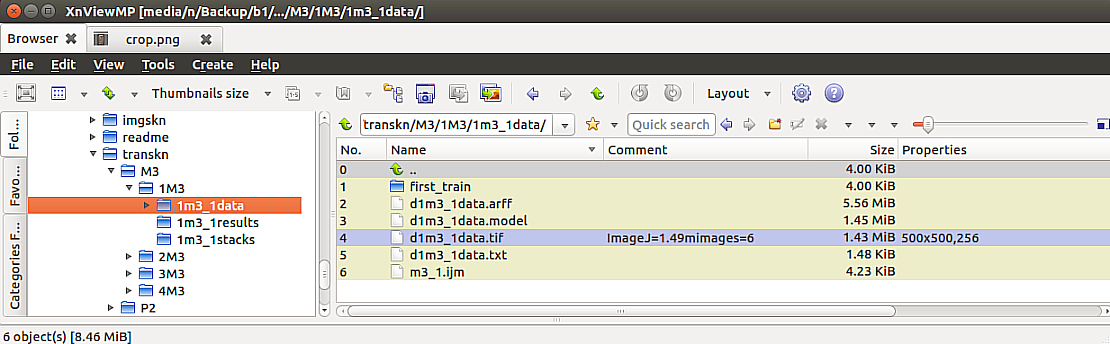
\includegraphics[width=1\linewidth]{gfx5/ctest/train-folder} \\
\caption[Classifier training and data folders.]{Classifier training and data folders}\label{fig:train-folder}
\end{figure}

Four training stacks were collated for each site. Each contained an image of the control grid (e.g. slice 2 for Mt. Tiger and Mt. Parihaka, and slice 1 for Memorial Drive) and an image of the inactive nest (acquired May 21 2013). Slices were arranged in date sequence. Each site-grid classifier was trained separately using respective stacks. There were twelve stacks in total, four per site. For each site, the first grid was used to train initial classifiers. A \emph{minimum} number of pixels were selected for each class label, starting with the control grid, and inactive grid slices. The segmentation results were checked and when they were satisfactory the grid$_{n}$.arff results were saved. The grid$_{n}$.arff files were loaded for the second grid classifier and training was run \emph{before} any new annotations were added. Results were checked and only where minimally necessary, new class traces were assigned to correct for segmentation inaccuracies. A new classifier was trained based on added class traces, saved and loaded into the next grid-batch classifier training. This process was repeated until all four grids were trained and checked across all site-grid training stacks. The final classifier for each site included the training across all four grids loaded as single final.arff data file. This classifier was applied to all image stacks for respective sties for final segmentation results. The training procedure is summarised as follows:

\begin{enumerate}
\item General training set-up procedures:
	\begin{enumerate}
	\item \ac{Fiji} \emph{Record Macro} was initiated to record all trace samples during training.
	\item \emph{Record Macro} files from each training session were saved for records as .ijm files and stored in site classification data folders (i.e. Folder 181\_classifiers\_~data/~transkn/~M3/~1M3/).
	\item Only those nests that could be clearly identified as active were used for class\_1 traces. 
	\item Only those areas that were clearly backgrounds were used for class\_2 traces.
	\item No attempt was made to try and equalise the class-data by providing the classifier with same number of traces for each class.
	\item Each of the three site-classifiers were trained using exactly the same general procedure outlined below.
	\end{enumerate}
\item Grid-training procedure:
	\begin{enumerate}
	\item Pixels were selected from the control and inactive images slices and these traces were automated with a \ac{Fiji} macro script.
	\item The script was applied to train an initial classifier.
			\begin{enumerate}
			\item No other traces were added; the initial base classifier was trained using only the automated annotations.
			\end{enumerate}
	\item After the first training-run the segmentation results were checked.
			\begin{enumerate}
			\item A \emph{very small} number of inaccurate segmentations, on a single image slice, were assigned to the correct classes with new traces. 
			\end{enumerate}
	\item The classifier was retrained and segmentation results were checked.
	\item If segmentations were still not accurate then a very small number of traces were reassigned, on a single slice and the classifier was retrained.
	\item If segmentation results deteriorated then the traces added during the previous training-run were removed. 
			\begin{enumerate}
			\item Another trace was added, at different location, and the classifier was retrained.
			\end{enumerate}
	\item This process was repeated sequentially until all slices were either annotated and/or properly segmented.
	\end{enumerate}
\item Site-training sequence:
		\begin{enumerate}
			\item Two training runs were used. 
			\item First-train data were saved into grid-data subfolders as shown in Figure \ref{fig:train-folder} above.
		\end{enumerate}
		\begin{enumerate}
			\item Each site-grid classifier were trained sequentially.
			\item Data from the initial grid-training (G1) were loaded into training for the next grid (G2).
			\item Start G2 first-training run:
				\begin{enumerate}
				\item Load Gf$ _{1}$.arff and train.
				\item Check segmentations and follow procedures 2 above to correct for any inconsistencies.
				\item Save Gf$_{2}$.arff
				\end{enumerate}
			\item The procedure was repeated until all site-grid classifiers were trained.
			\item Final annotations were saved as final.arff data.
		\end{enumerate}
			\item Application of final site-classifier to monitoring data:
			\begin{enumerate}
			\item Data (final-site.arff) and classifier model (final-site.model) from site-training was loaded into \ac{TWS}.
				\begin{enumerate}
					\item Grid monitoring stacks were selected in sequential order.
					\item The classifier was applied as a batch process.
					\item Binary results and data were saved to grid folders and subfolders.
				\end{enumerate}
			\end{enumerate}
\end{enumerate}

\section{Post-processing}\label{sec:post-processing}

Several morphological operations and pipeline combinations were empirically tested using the small test stack. When the morphological operations were completed the counted results were visually checked against the original \ac{RGB} images, and against the values recorded for manual field counts. The post-processing method was automated in a script (Listing \ref{cd:pp}) and applied in as a batch process. The procedures used in the post-processing pipeline are detailed below. They include the binary options settings, the morphological operators used and object descriptors used for final binary counts. 

\begin{enumerate}
\item Binary options and final settings. Refer to Figure  \ref{fig:binary-particles-options} (a) below.
	\begin{enumerate}
	\item Iterations: 
		\begin{enumerate}
		\item Specifies the number of times operations are performed.
		\end{enumerate}
	\item Count:
		\begin{enumerate}
		\item The number of adjacent background pixels necessary before they are removed from the edge of objects during the erosions.
		\item The number of adjacent foreground pixels necessary before pixels are added to the edge of objects during dilation\footnote{\label{note1}see http://imagejdocu.tudor.lu/doku.php?id=gui:process:binary}..
		\end{enumerate}
	\item Pad edges:
		\begin{enumerate}
		\item Setting was checked for all post-processing operations.
		\item Affects eroding and closing.
		\item Edge erosion was not performed during\\ \emph{Process>Binary>Erode} and\\ \emph{Process>Binary>Close}\textsuperscript{\ref{note1}}.
		\end{enumerate}
	\item EDM output was checked to overwrite the 8-bit input images\textsuperscript{\ref{note1}}.
	\end{enumerate}
\item Post-processing pipeline:
	\begin{enumerate}
		\item \emph{Fill Holes}
			\begin{enumerate}
			\item Filled holes in binary objects.
			\end{enumerate}
		\item \emph{Close}: 10 iterations 5 counts. 
			\begin{enumerate}
			\item Dilations\footnote{Dilate: enlarges object borders so holes become smaller.} followed by erosions\footnote{Erode: shrinks the image so holes became larger and small details are deleted.}. 
			\item Connected any disconnected parts of the binary images
			\item Joined breaks, closed holes and smoothed out contours.
			\end{enumerate}
		\item \emph{Fill Holes}
			\begin{enumerate}
			\item Filled any remaining holes.
			\end{enumerate}
		\item \emph{Open}: 2 iterations 3 counts. 
			\begin{enumerate}
			\item Erosion followed by dilation.
			\item Separated connected objects in the images.
			\item Smoothed contours removing isolated objects. 
			\end{enumerate}
	\end{enumerate}
\item  Analyze Particles for three binary schemes. Refer to Figure  \ref{fig:binary-particles-options} (b) below. 
	\begin{enumerate}
	\item Analyze Particles options:
	\item \emph{Circularity} was set between $0.10-1.00$ for all schemes.
	\item \emph{Pixel sizes} ($ p^2$):
		\begin{enumerate}
		\item $ p^2 = 10-\infty$
		\item $ p^2 = 15-\infty$
		\item $ p^2 = 20-\infty$
		\end{enumerate}
	\item \emph{Image Overlay} was checked to create a separate overlay image stack showing the outlines of counted objects. Refer to Figure  \ref{fig:binary-particles-options} (c) below. 
	\end{enumerate}
\item \emph{The final binary counts}:
	\begin{enumerate}
	\item The average count over the three binary schemes.
	\item The median values over three image collections.
	\end{enumerate}
\item Post-processing macro snippet:
\begin{lstlisting}[language=java, caption=Post-processing snippet., label=cd:pp]
//open classified image stacks and post-process
run("Make Binary", "method=Default background=Default calculate");
run("Options...", "iterations=1 count=1 edm=Overwrite do=[Fill Holes] stack");
run("Options...", "iterations=10 count=5 pad edm=Overwrite do=Close stack");
run("Options...", "iterations=1 count=1 edm=Overwrite do=[Fill Holes] stack");
run("Options...", "iterations=2 count=3 pad edm=Overwrite do=Open stack");
//count nests using three schemes....
run("Analyze Particles...","size=10-Infinity circularity=0.10-1.00 show=[Overlay Outlines]
run("Analyze Particles...","size=15-Infinity circularity=0.10-1.00 show=[Overlay Outlines]
run("Analyze Particles...","size=20-Infinity circularity=0.10-1.00 show=[Overlay Outlines]
\end{lstlisting}
\end{enumerate}

\begin{figure}[!htbp]\myfloatalign
\subfloat[Binary options.]{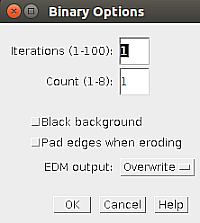
\includegraphics[width=.3\linewidth]{gfx5/post/binary-options}}\
\subfloat[Analyze Particles.]{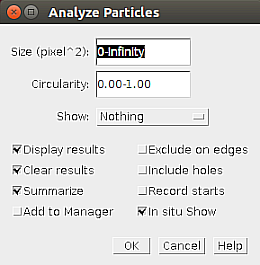
\includegraphics[width=.4\linewidth]{gfx5/post/particles-options}} \\
\subfloat[Example of binary count overlays in a pdf file.]{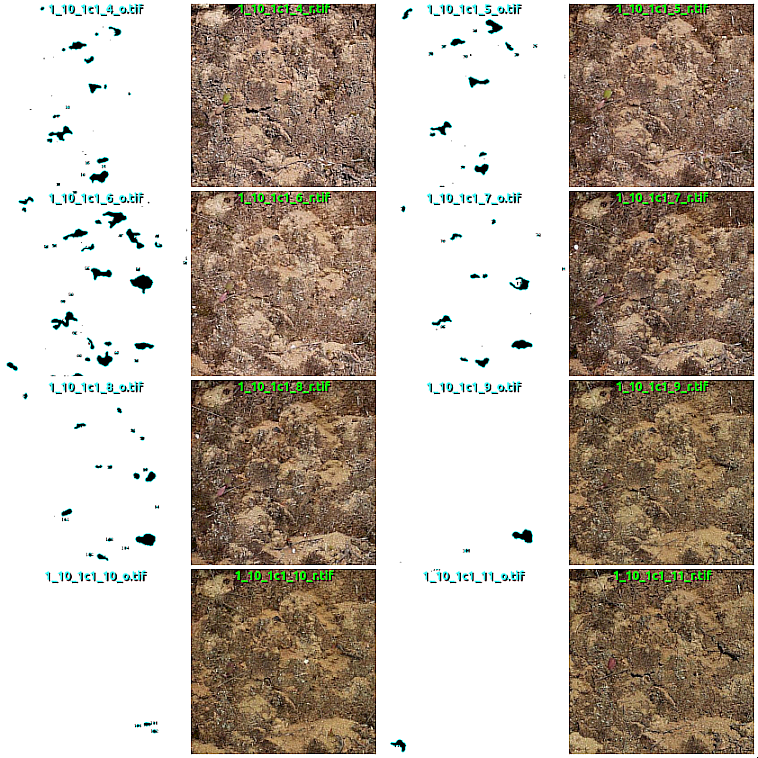
\includegraphics[width=.8\linewidth]{gfx5/post/binary-count}} 
\caption[Binary options interface.]{Post-processing operators in Fiji. The user interface to select the (a) Binary options and morphological operators applied to segmented images. The settings used to count binary objects in images with the (b) Analyze Particles utility. The binary count overlays (c) which were manually checked against raw \ac{RGB} images for accuracy.}\label{fig:binary-particles-options}
\end{figure}

\section{Classical segmentation methods} 


\subsection{Thresholding monitoring images}
Raw monitoring images were collated into a single stack. The default binary threshold was applied to the stack and it was post-processed using the operators and settings outlined above. The count results were imported into the monitoring spreadsheet and used for comparative analysis between automatic counts derived from thresholding and those from segmentations using the CF classifier. Post-processed images with count overlays were collated alongside raw image slices into a single stack. The stack was saved as a pdf document for manual checking and reporting. 

\section{Manual counts from images}
Images for manual counts were randomly selected from image data using the spreadsheet list. One hundred and seventy images were used for manual image counts. They were collated into a single pdf stack. Another stack was created which included counted overlay results; this stack was used for verification (Figure \ref{fig:binary-particles-options} (c)). Two observers conducted counts on the raw \ac{RGB} images. Scorers reviewed which objects could realistically be identified as active nests after a trial run. 
Final counts were conducted in a complete run with no further discussions. The first sequence was carried out by the first scorer, followed by the second. Data were entered directly into a spreadsheet by one scorer, as counts were made by the other. Counts were made as quickly as possible. The process was repeated three times by each scorer. The mean counts for each observer were taken and rounded up to whole numbers. These were used in final comparative analysis between the three methods. The manual image count procedure is summarised as follows:

\begin{enumerate}
\item Images were randomly selected but only from paired-monitoring data (i.e ND filler images were not included).
	\begin{enumerate}
	\item Raw \ac{RGB} images were compiled into a single pdf document as shown in Figure \ref{fig:binary-particles-options}.
	\item Images were compiled in sequential order and labelled with file reference identifiers as image overlays.
	\item Trial nests counts from image data:
		\begin{enumerate}
		\item A trial nest count from images was made by two observers.
		\item Discussions between observers were conducted regarding the images.
		\item This was to determine what objects could be reasonably reconsigned as active nests.
		\item After reasonable agreement between observers were reached manual nest counts from images were collected.
		\end{enumerate}
	\item Manual nest counts from image data:
		\begin{enumerate}
		\item There were no further discussions between observers about nest images when counts were conducted.
		\item Counts were made from pdf images in a single complete run.
		\item Each scorer conducted three replica counts in turn.
		\item While one scorer counted, the other recorded data immediately to a spreadsheet.
		\end{enumerate}
	\end{enumerate}
\item A corresponding pdf comprising of raw \ac{RGB} images alongside automatic count overlays were compiled into a corresponding pdf (Figure \ref{fig:binary-particles-options} (c)).
\item If required, verification of manual-image counts could be checked alongside raw RBG images and automatic nest count overlays.
\end{enumerate}


\section{Data preparation and analyses}\label{sec:data-preparation-for-analyses}
Each image collection was comprised of near-replica images. They were data collected from the same location, grid and day but separated by minutes:seconds. Separate collections were therefore comprised of different images; each single one was acquired under varying natural conditions. Therefore \emph{median counts} were taken across three image collections. Count data for all methods were prepared in spreadsheets as follows:

\begin{enumerate}
\item For automatic nest count data.
	\begin{enumerate}
	\item Image collections (C1-C3).
		\begin{enumerate}
		\item The mean nest counts from three binary schemes were calculated. 
		\item Values were rounded up to whole numbers to provide automatic-count subtotals.
		\end{enumerate}
	\item The median counts from three image collections on the were taken on the automatic-count subtotals. 
	\item This provided the final automatic-count data used in comparative method analysis (the CF classifier--\emph{ac} and threshold method--\emph{at}).
	\end{enumerate}
\item For manual-image count data.
	\begin{enumerate}
	\item The mean of three replica counts were taken for each observer and rounded up to whole numbers.
		\begin{enumerate} 
		\item This provided manual-image count data (\emph{mic\_ob1 and mic\_ob1}).
		\item Data were used for inter-observational analysis.
		\end{enumerate}
	\item The mean counts from two observers were taken and round to up whole numbers. 
	\item This provided the final manual-image data used for comparative method analysis (\emph{mic\_t}).
	\end{enumerate}
\item For manual-field count data.
	\begin{enumerate}
	\item The mean of three replica counts were taken for both observers round up to whole numbers. 
	\item These provided the manual-field data used in comparative method analysis (\emph{mfc\_t}).
	\end{enumerate}
\end{enumerate}

\subsection{Methods comparisons}\label{sec:methods-comparisons}
Verification of the image-centric method focused on five primary comparative assessments:

\begin{enumerate}
\item Automated counts from the \ac{RF} optimised model (ac) and classical thresholding (at).
\item Manual counts from the images by two observers (mic\_ob1 and mic\_ob2.
\item Manual counts from the images (mic) and from the field (mfc).
\item Automated counts from the \ac{RF} optimised model (ac) and manual from the images (mic). 
\item Automated counts from the \ac{RF} optimised model (ac) and manual counts from the field (mfc). 
\end{enumerate}

\begin{figure}[!htbp]\myfloatalign
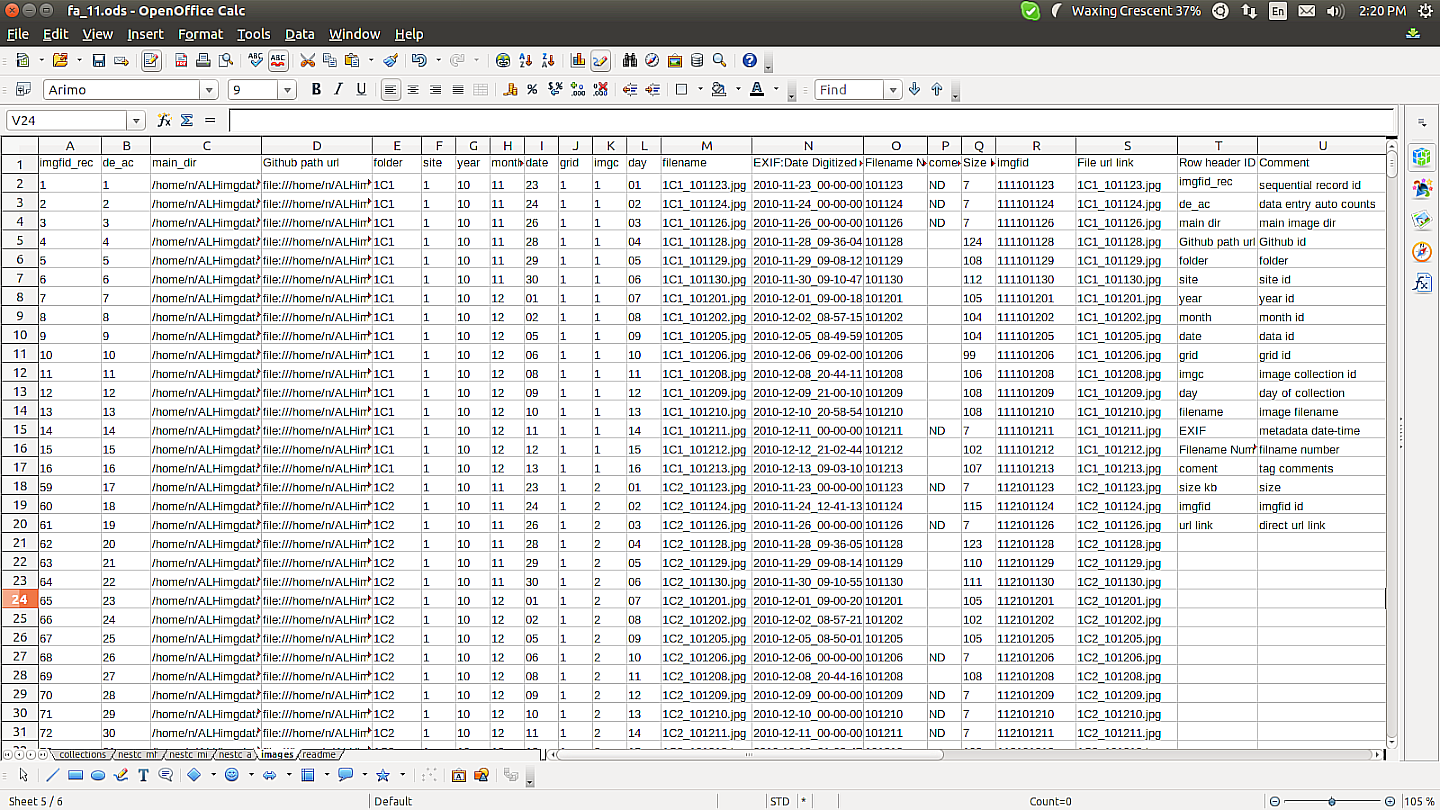
\includegraphics[width=1\linewidth]{gfx5/post/csv-data-imagefiles} \\
\caption[Image data files.]{The images data sheet shown was one of six used for monitoring data entry: collections (basic records), 2) nestc\_mf (manual-field counts), 3) nestc\_mi (manual-image counts), 4) auto\_c (automatic counts), 5) images (image data files and hard links) and 6) readme (row header descriptions).}\label{fig:data-entry}
\end{figure}

Statistical analysis were performed in R-Studio. They were formatted in spreadsheets to accommodate easy import. Data were organised using a single header row and arranged using date-time or grid-image sequences in single long columns. Examples are shown in Figure \ref{fig:data-entry}. The first column for each sheet contained a sequential base reference identification. All zero count data were input as $0$; all \emph{no-data} entries were identified by a text value entered as \emph{ND} as demonstrated in \ref{fig:data-entry} column P--comments.

\subsection{Statistical tests}\label{sec:statistical-data-analyses}
Lin's Concordance of Correlation ($ \rho_c $) was used to compare methods. It combines measures of accuracy and precision to test the agreement (or accuracy) between two observations \cite{Lin1989}.In the equation $ \rho_c = rC_b $ and $ r $ is the correlation coefficient and $ C_b $ is determined by:
\[ C_b = [\dfrac{(\nu + 1/\nu + u^{2})}{2}]^-1 \] \\
Here:\\
$ \nu = \sigma_{x} /\sigma_{y} $ where $\sigma $ is the variance of $x$ and $y$\\
$ \mu $ is the mean value of $ x $ and $ y $ respectively \\
$ u = (\mu_{x}-\mu_{y})/\sqrt{\sigma_{c}\sigma_{y}} $ \\

Pearson's correlation coefficient $r$ shows how scattered the data points are around the line of best fit and gives a \emph{measure of precision}. The value of $ \mu $ defines the scale shift and measures systematic bias in measured values compared with actual values; $ \nu $ defines the location shift and measures the difference between actual and measured values; and $ C_{b} $ is a bias correction factor calculated using $ \nu $ and $ \mu $. $ C_{b} $ gives a \emph{measure of accuracy}. A \emph{perfect concordance} between actual and measured values would return $\rho_{c}= 1$, $r = 1$, $C_{b} = 1$, $\nu  = 1$, and $\mu = 0$. 

The value $ \rho_c $ was calculated using the epi.ccc function in the epiR package \cite{stevenson2012}. The R-studio graphical user interface is shown in Figure \ref{fig:rstudio} and the epi.ccc function is demonstrated in Listing \ref{cd:rstudio} below. Graphical analyses were saved as results.tiff for records; a notebook was compiled from the R script associated with each analysis and saved as a pdf.

\begin{figure}[!htbp]\myfloatalign
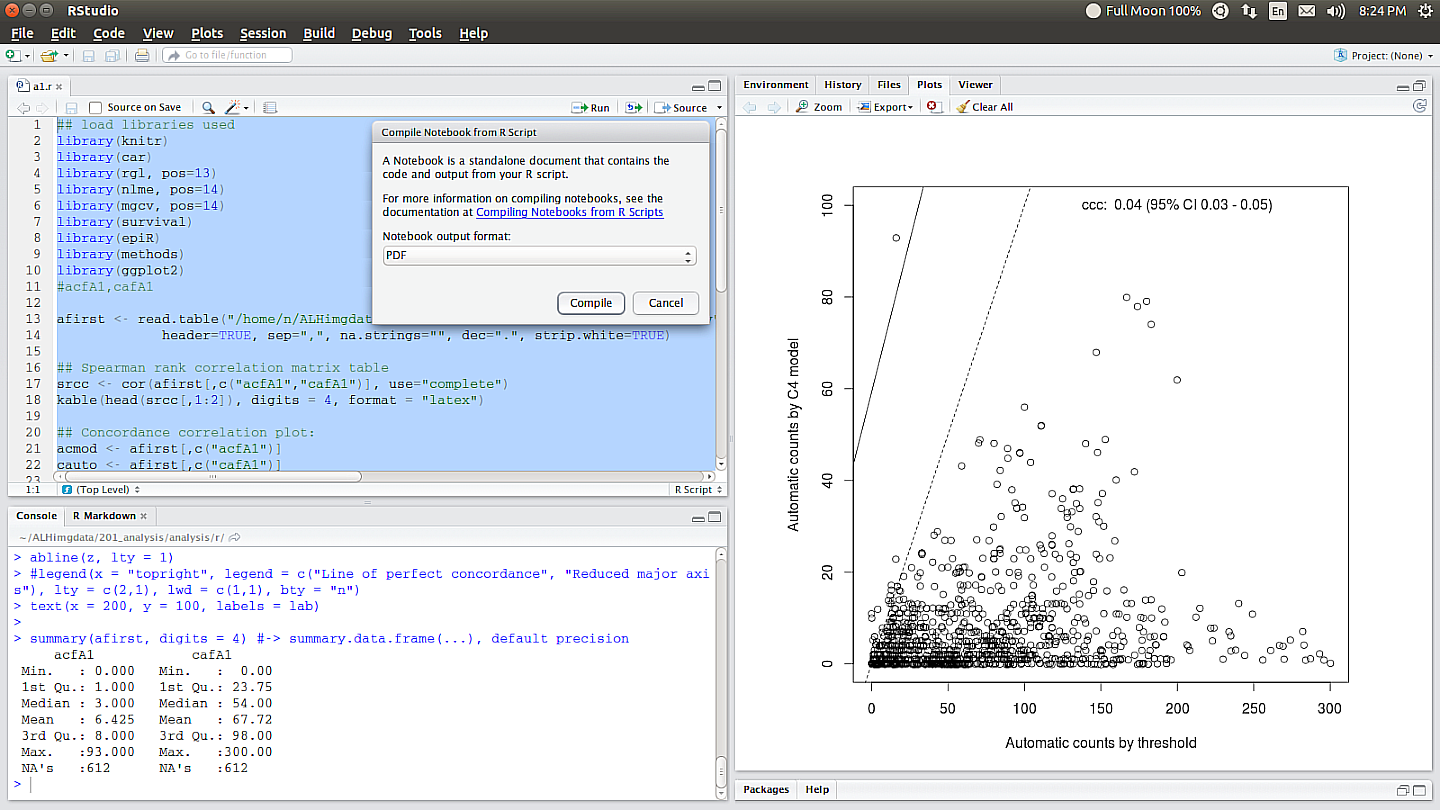
\includegraphics[width=1\linewidth]{gfx5/ctest/rstudio} \\
\caption[R-Studio interface for statistical analysis.]{R-Studio graphical user interface showing the operation of the script in Listing \ref{cd:rstudio} below}\label{fig:rstudio}
\end{figure}

\begin{lstlisting}[float, language=r, caption={[R-studio concordance correlation script.]R-studio concordance correlation script for automatic counts by thresholding and the CF classifier.}, label=cd:rstudio]
## load libraries used
library(knitr)
library(car)
library(rgl, pos=13)
library(nlme, pos=14)
library(mgcv, pos=14)
library(survival)
library(epiR)
library(methods)
library(ggplot2)
afirst <- read.table("/300_documents/ch6_imgs/finals/rA1/A1.csv", 
             header=TRUE, sep=",", na.strings="", dec=".", strip.white=TRUE)
## Spearman rank correlation matrix table
srcc <- cor(afirst[,c("acfA1","cafA1")], use="complete")
kable(head(srcc[,1:2]), digits = 4, format = "latex")
## Concordance correlation plot:
acmod <- afirst[,c("acfA1")]
cauto <- afirst[,c("cafA1")]
## cc correlation matrix table
cccfirst <- epi.ccc(cauto, acmod, ci = "z-transform", conf.level = 0.95)
firstr <- cccfirst$rho.c
kable(head(firstr[,1:3]), digits = 4, format = "latex")
tmpfirst <- epi.ccc(cauto, acmod, ci = "z-transform",conf.level = 0.95)
lab <- paste("ccc:  ", round(tmpfirst$rho.c[,1], digits = 2), " (95% CI ", 
             round(tmpfirst$rho.c[,2], digits = 2), " - ",
             round(tmpfirst$rho.c[,3], digits = 2), ")", sep = "")
z <- lm(cauto~acmod)
par(pty = "s")
plot(jitter(cauto),jitter(acmod), xlim = c(0, 300), ylim = c(0,100), cex=1, xlab = "Automatic counts by threshold", ylab = "Automatic counts by CF model", pch = 1) abline(a = 0, b = 1, lty = 2) abline(z, lty = 1)
text(x = 200, y = 100, labels = lab)
\end{lstlisting}

\section{Summary of imaging methods}\label{sec:summary-of-imaging-methods}
Substantial Chapter.
Image data management.
Software tools and methods
Machine learning 
Classifier optimisation and tuning
Feature engineering
Trees and random features
Data handling and final preparations
Statistical analysis
Concentrate on methods - not classifier performance
